%!TEX root = ../../main.tex
\section{RSConverter}
RS485-bussen er valgt til at kommunikere på, se hvorfor i teknologiundersøgelsen. Til dette formål er udformet et simpelt kredsløb vha. MAX3082. Det logiske 0-5V UART-signal fra PSoC 4 konverteres til et differentielt signal, som kører ud på bussen, og vice versa.

\begin{figure}[H]
	\centering
	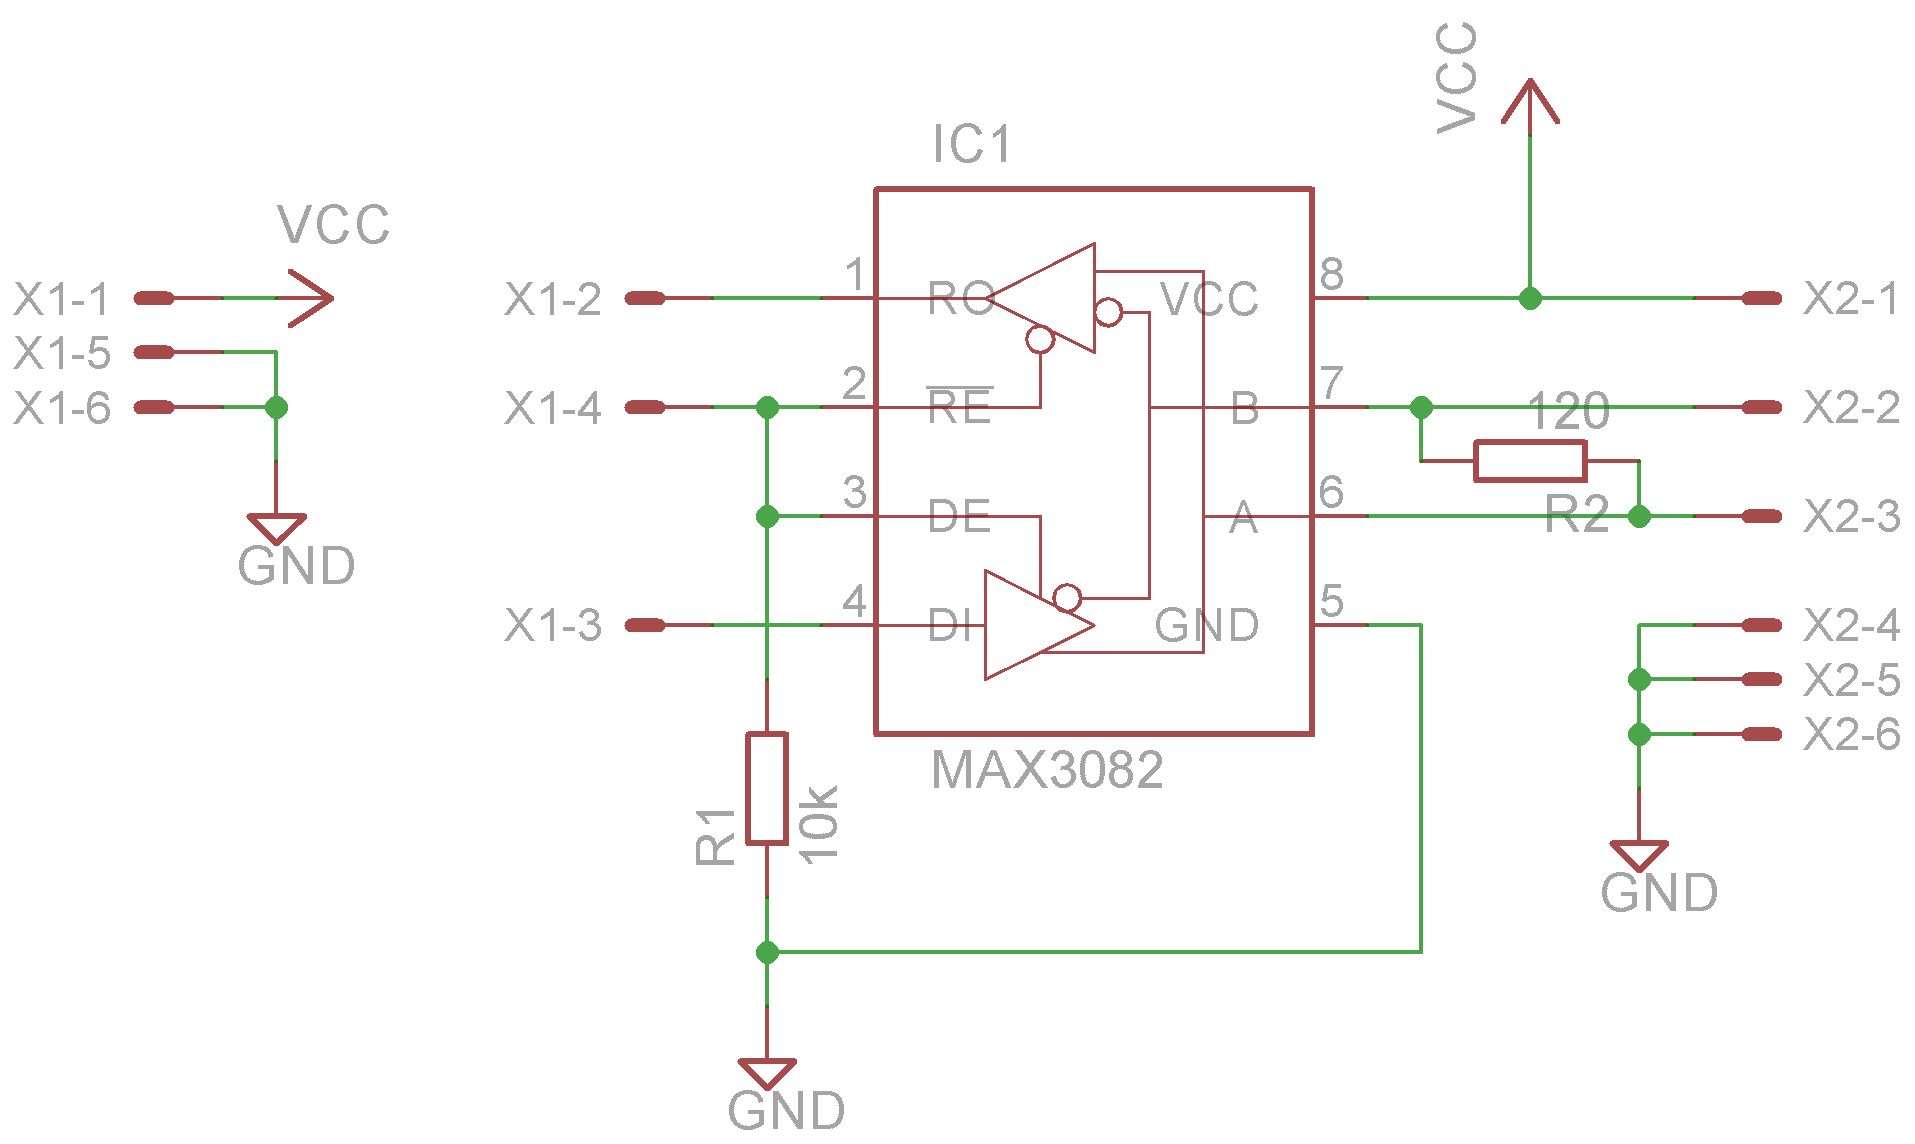
\includegraphics[scale=1]{../Hardware/RS485_Converter/Schematic}
	\caption{RS485 converter}
	\label{photo:RS485converter}
\end{figure}

\fxnote{Scopebilleder, forklaringer osv.}